
\title{Introduction}

%\section{List of abbrevations}
%KDA = Kongsberg Defence \& Aerospace \\
%SBC = Single Board Computer



\section{Introduction}

We are a team of six computer engineering students from the University of South-Eastern Norway, Campus Kongsberg. Our bachelor assignment was given to us by Kongsberg Defence \& Aerospace (KDA), a Norwegian technology company headquartered in Kongsberg. KDA specializes in manufacturing equipment for defense, space exploration, and aviation.\cite{KongsbergGruppen}\\

Our client conducts a student-centered initiative known as 'Local Hawk', which is operational during the summer. The main focus of this initiative is to investigate a variety of methods for fostering the development of autonomous drones. The client has expressed an interest in our project with the aim of garnering insightful data that could be applied to future deliberations concerning the architectural design of these unmanned aerial vehicles, with special emphasis on Frames-Per-Second (FPS), as this is the most crucial and important aspect.\\


The drone systems traditionally used in the Local Hawk project has limited computing power and restrictions on weight. KDA expressed an interest in doing a research project for our assignment, where we would examine any potential performance gains by moving the processing closer to the sensor hardware, meaning we will be using dedicated hardware for image processing.\\

\section{Problem Domain}

The drones being used in the Local Hawk project today use what we call Single Board
Computers (SBC). These devices are usually created in a small form factor, and due to their limited size, they are also limited in processing capabilities. This means that it has challenges performing several tasks simultaneously, e.g., controlling the drone motors and executing object detection at the same time. \\

In earlier iterations of Local Hawk they attempted to run object detection while flying the drone at the same time on a single SBC. This resulted in very low framerate which in turn meant that it could not be used for any meaningful purpose. The reason for this is that processing camera images can be computationally expensive. For instance, if we need to process a 24-bit color image with a 600x600 resolution pixel-by-pixel, we would have to handle 360,000 pixels, each with 3 color channels, resulting in an input data size of 1,080,000 bytes per image. This poses a challenge for the limited hardware available for a lightweight drone. \\

%Real-time object detection is a common task for autonomous vehicles. An object detection algorithm can both classify predefined objects in an image and output the location of classified objects within the image. Real-time object detection requires the system to run the image input through complex algorithms multiple times per second.
%The hardware required to perform real-time object detection is widely available today in the form of consumer-grade CPUs and GPUs. However, a problem arises if the autonomous vehicle has any restrictions on weight, physical space, and power consumption, which is the case with small Unmanned Aerial Vehicles (UAVs). \\


%Cameras are a common choice for sensors in autonomous vehicles due to their versatility, low cost, and potential. However, one downside is that processing camera images can be computationally expensive. For instance, if we need to process a 24-bit color image with a 600x600 resolution pixel-by-pixel, we would have to handle 360,000 pixels, each with 3 color channels, resulting in an input data size of 1,080,000 bytes per image. Real-time object detection is a common task for autonomous vehicles. An object detection algorithm can both classify predefined objects in an image and output the location of classified objects within the image. Real-time object detection requires the system to run the image input through complex algorithms multiple times per second.

%The hardware required to perform real-time object detection is widely available today in the form of consumer-grade CPUs and GPUs. However, a problem arises if the autonomous vehicle has any restrictions on weight, physical space, and power consumption, which is the case with small Unmanned Aerial Vehicles (UAVs). \\

%In previous years, the participants of KDA’s Local Hawk summer project have attempted to run object detection on a lightweight UAV. Their attempts had a detection framerate of around 1 frame per second and this showed that an unaccelerated approach is not conductive for any meaningful functionality. Their results were achieved by using a single Raspberry Pi 4 for all the UAV’s computations.

The primary objective of this study is to meticulously evaluate various software and hardware architectures for a compact UAV equipped with object detection capabilities. We will place a particular emphasis on identifying the potential frames-per-second (FPS) improvements attainable on our systems, as this is our main focus. Each architecture will be critically analyzed and compared based on parameters such as performance, cost, complexity, and weight.\\

While the aspiration of implementing these architectures in an actual UAV or drone system is considered a secondary or stretch goal, the core of our research will provide valuable insights and recommendations. These recommendations will cater to the technology selection process when designing lightweight UAVs for diverse applications requiring object detection capabilities. By doing so, our findings are expected to significantly contribute to the design of efficient and effective UAV systems.\\

In the context of the Local Hawk project, image processing is particularly essential when considering the use case of "Autonomous Landing". UAVs operate in diverse environments with various terrains and conditions, making precise and safe landings a challenge. Through image processing, the drone can significantly enhance its autonomous landing capabilities. One such improvement is the incorporation of visual markers to indicate the designated landing spot. By identifying these markers, the drone can ascertain the designated landing spot, ensuring a more precise and controlled landing.

\section{Research Perspective}

In our initial discussions with the client, it was clearly communicated that they desired a research report containing actionable information for decision-making, provided our findings indicate the potential for a successful endeavor.\\

This presented challenges for us, as we lacked prior experience with research-focused projects. Consequently, we needed to adapt our approach in order to comprehend how best to organize and execute our work, ensuring optimal delivery of results.\\

During the initial stages of the project, we deliberately refrained from immediately engaging with specific technologies or embarking on the development of a product in a domain where our knowledge was limited. Instead, we adopted a hermeneutic process, which is not commonly employed in engineering or systems engineering. However, this methodology proves valuable when dealing exclusively with knowledge and information, rather than specific implementations.\cite{Dialektikk} \\

The diagram of the hermeneutic spiral presented below illustrates the practical application of this concept. As our understanding of the problem domain deepens, we gained the ability to formulate more refined inquiries regarding the information that is relevant to us and the client. This enhanced understanding guided us in approaching the problem domain with the aim of achieving the desired results.\\

\begin{figure}[h]
    \centering
    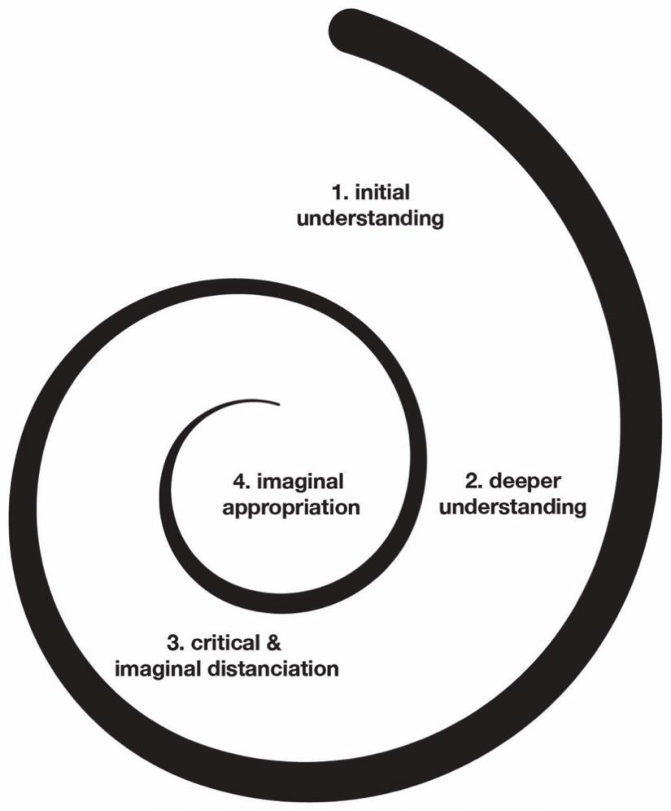
\includegraphics[scale=0.5]{fig/HS.png}
    \caption{Hermenutic Spiral \cite{hermeneutics}}
\end{figure}

%\section{Research Areas}

%The different configurations we presented as options to the client gives us ample opportunity to answer several questions raised by the limitations of the current design. We will investigate closer how the current design works, and then contrast that with our designs. This will allow us to compare speed in regards to frame per second on image processing, the advantages and disadvantages of a distributed approach contrasted with the central approach that exists today and possible limitations and disadvantages on a distributed approach, as it is likely we will not be able to say with absolute certainty that one approach fits all in every scenario.\\

%\section{intro 2.0?}

%Cameras are commonly used as sensors for autonomous vehicles due to their versatility, low cost and untapped potential. A downside is that doing something meaningful with camera images can be very computationally expensive. Let’s say we want to process a 24-bit color image with a 600x600 resolution pixel-by-pixel. That’s 360 000 pixels with 3 color channels each, giving us an input data size of 1 080 000 bytes per image. A common task for an autonomous vehicle is real-time object detection, which requires the system to run the image input through complex algorithms multiple times per second.

%The hardware required to perform real-time object detection is widely available today in the form of consumer-grade CPUs and GPUs. However, a problem arises if the autonomous vehicle has any restrictions on weight, physical space and power consumption, which is the case with small Unmanned Aerial Vehicles (UAV).

%In previous years, the participants of KDA’s Local Hawk summer project have attempted to run object detection on a lightweight UAV. Their attempts have not led anywhere as the detection framerate at around 1 frame per second was too low for any meaningful functionality. Their results were achieved by using a single Raspberry Pi 4 for all the UAV’s computations.

%This study aims to explore multiple software and hardware architectures for a small UAV with object detection capabilities. The configurations will be compared in terms of performance, cost, complexity and weight. Our results will provide recommendations on which technology to use when building lightweight UAVs for various use cases which require object detection.\\



%\subsection{Customer}

%The customer for this project was Kongsberg Gruppen, a local technology company with a global presence in the fields of defense, aerospace, maritime, and digital industries. \\

%The results of this project will be used in KDAs summer internship project “Local Hawk”, where they develop autonomous UAV (Unmanned Aerial Vehicles) over the summer. \\

%Throughout the duration of the project, Kongsberg Gruppen provided valuable insights, feedback, and guidance, which helped shape the project's direction and ensured its success. Regular meetings and communication with the customer allowed the team to stay aligned with their expectations and make any necessary adjustments to the project's scope and objectives. \\






\newpage

